\section{Analysis Results}

\subsection{Belt Drive}\label{sec:bd_fea}

\begin{figure}[H]
\centering
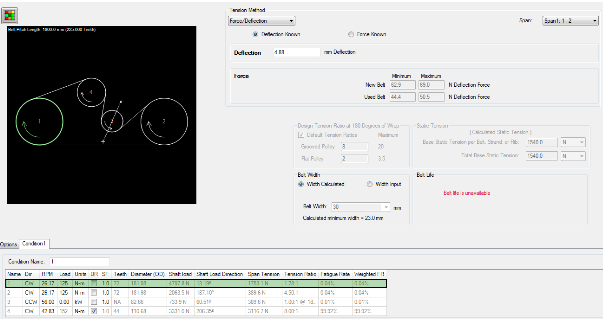
\includegraphics[width=\textwidth]{images/drive_analysis}
\caption[Drive Analysis]{Drive analysis using the Gates Design IQ software.}
\label{fig:drive_analysis}
\end{figure}

\begin{figure}[H]
\centering
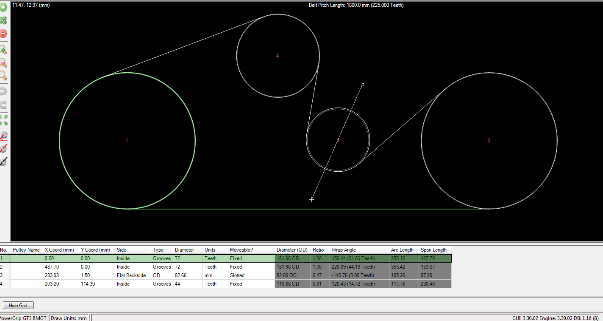
\includegraphics[width=\textwidth]{images/drive_layout}
\caption[Drive Layout]{Drive layout using the Gates Design IQ software.}
\label{fig:drive_layout}
\end{figure}

\subsection{Wheel Shaft}\label{sec:ws_fea}

\begin{figure}[H]
	\centering
	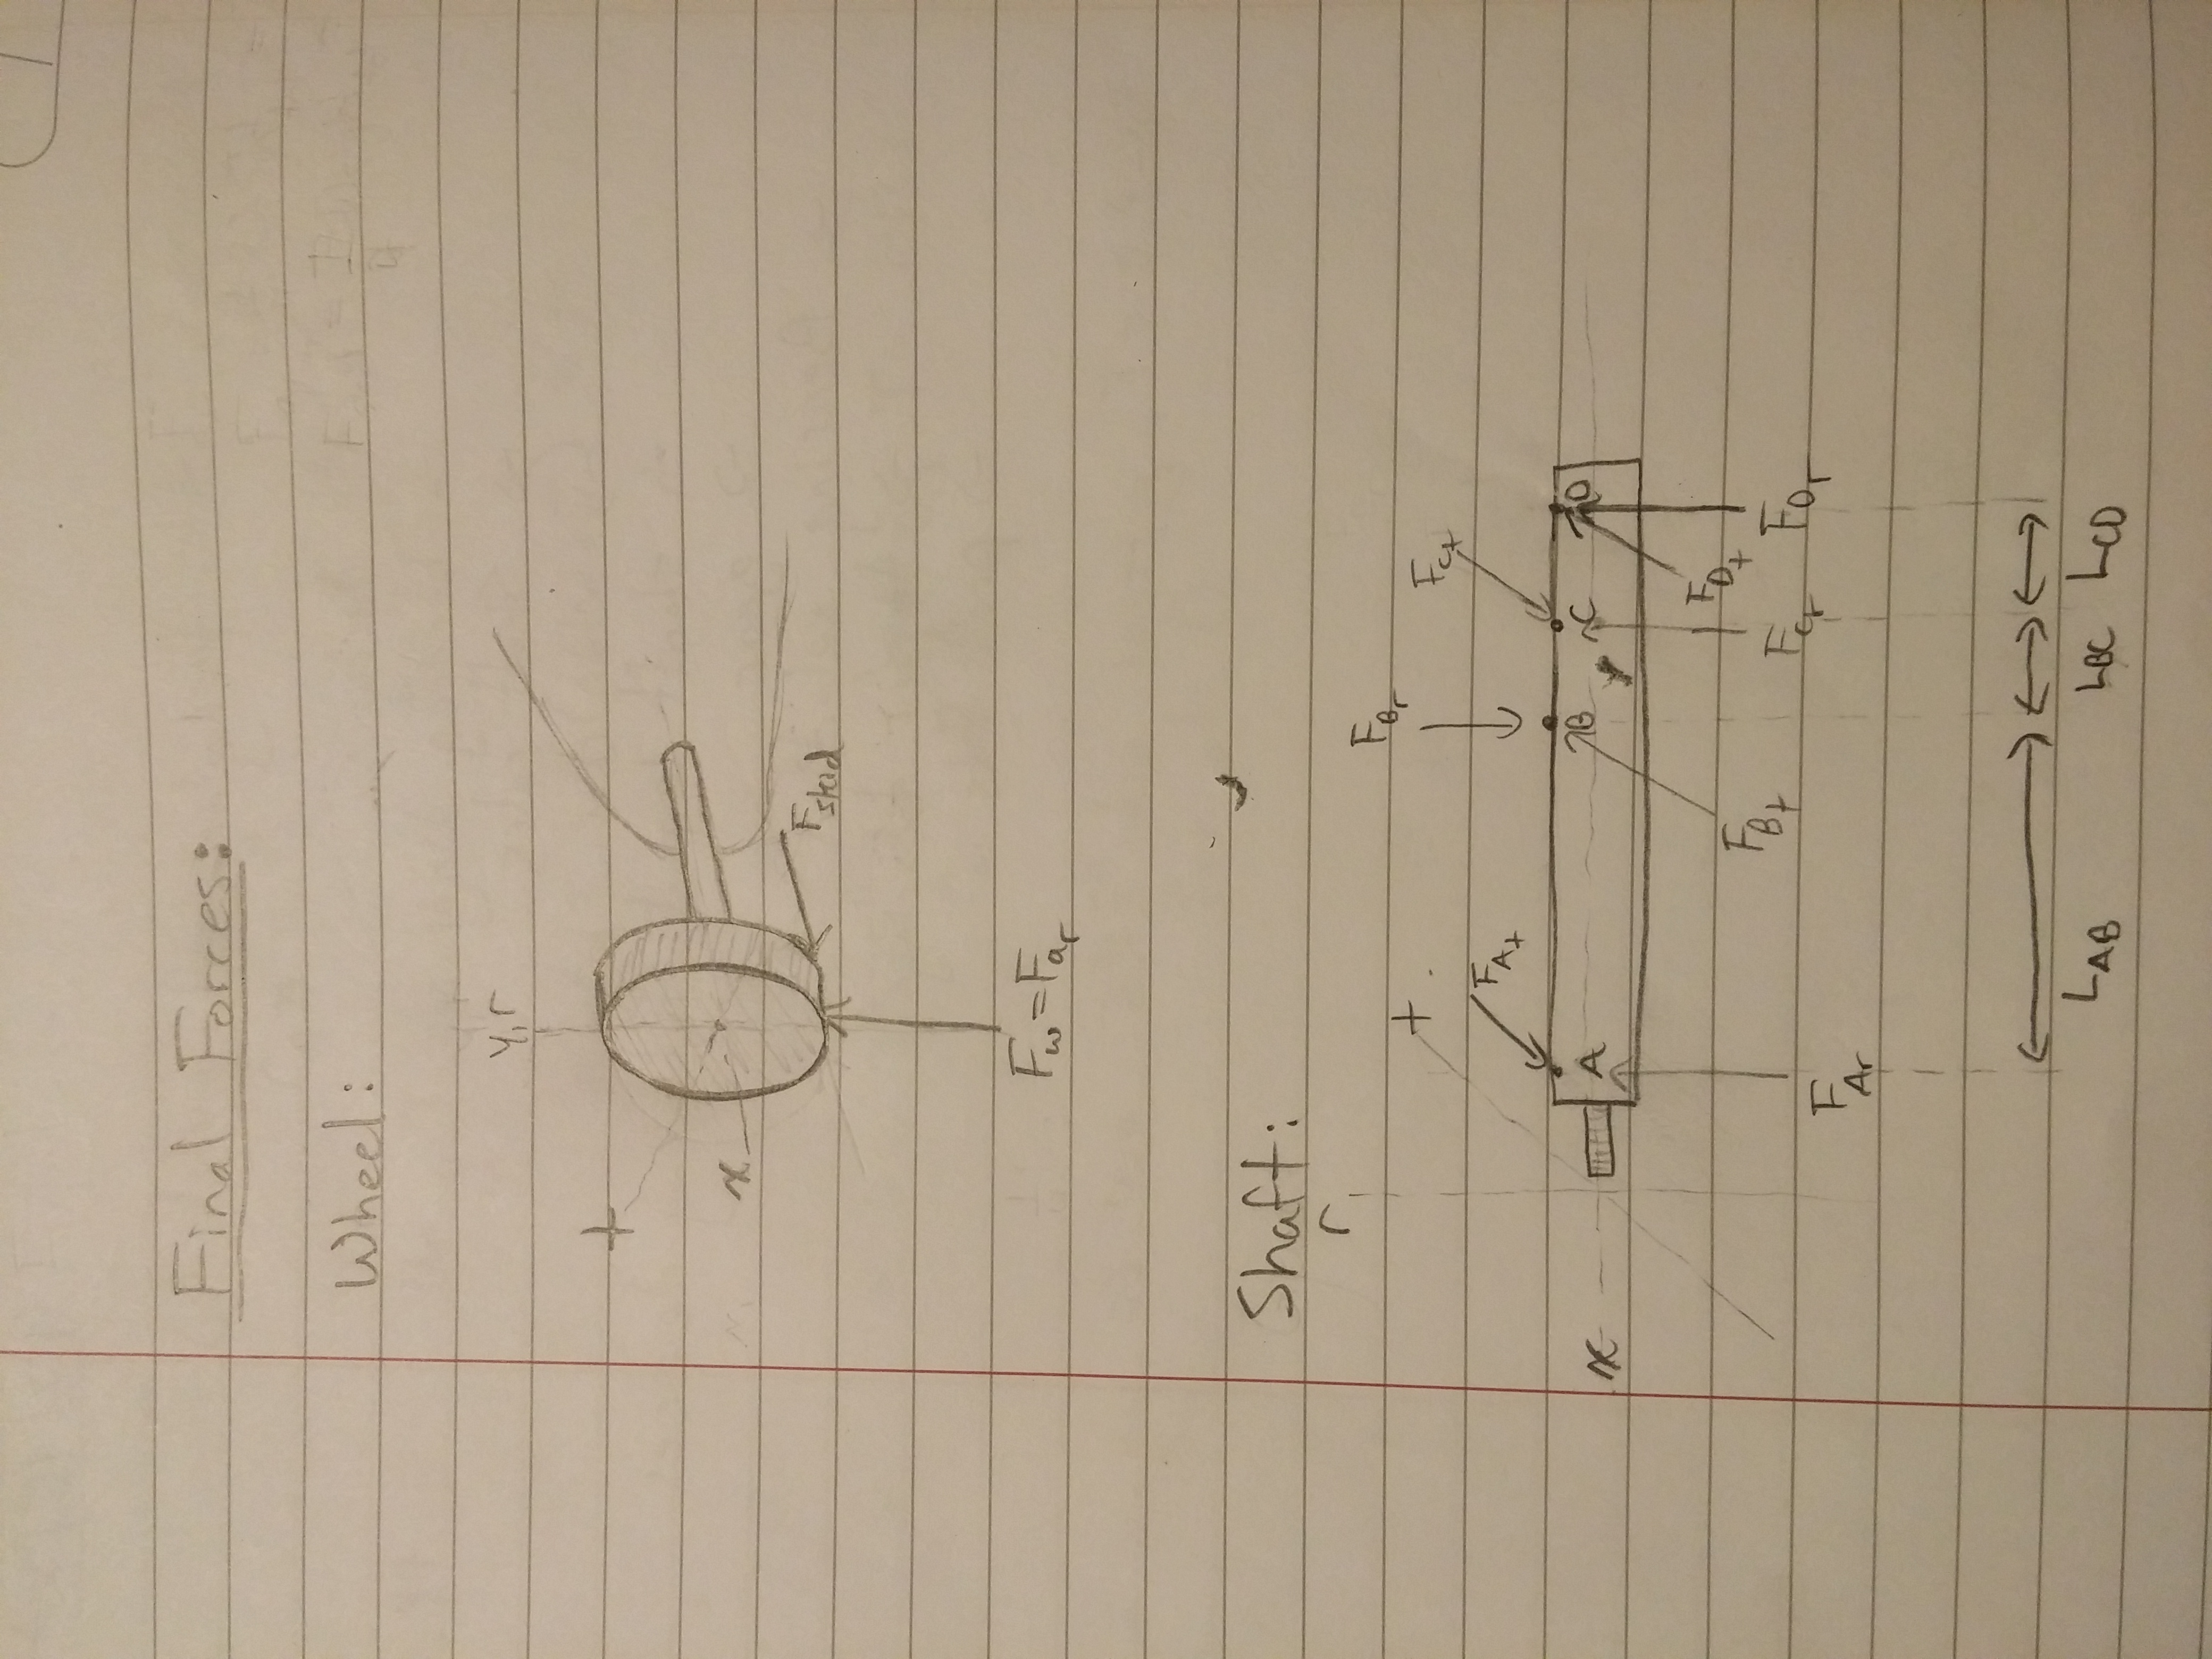
\includegraphics[width=\textwidth]{dom/loading_conditions_calc.jpg}
	\caption{FBD of loading conditions for wheel shaft.}
	\label{fig:fbd_wheelshaft}
\end{figure}

\begin{figure}[H]
\centering
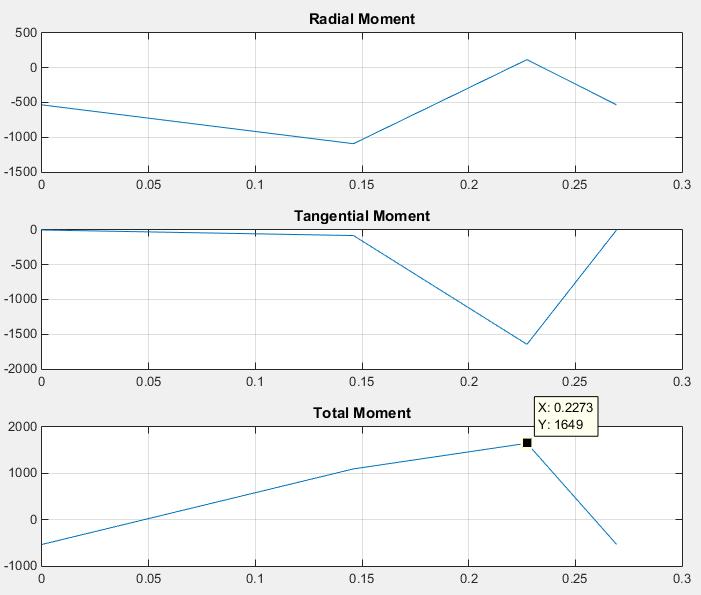
\includegraphics[width=\textwidth]{images/wheelshaft_bmd}
\caption{Wheel Shaft Bending Moment Diagram}
\label{fig:wheel_shaft_bmd}
\end{figure}

\begin{figure}[H]
	\centering
	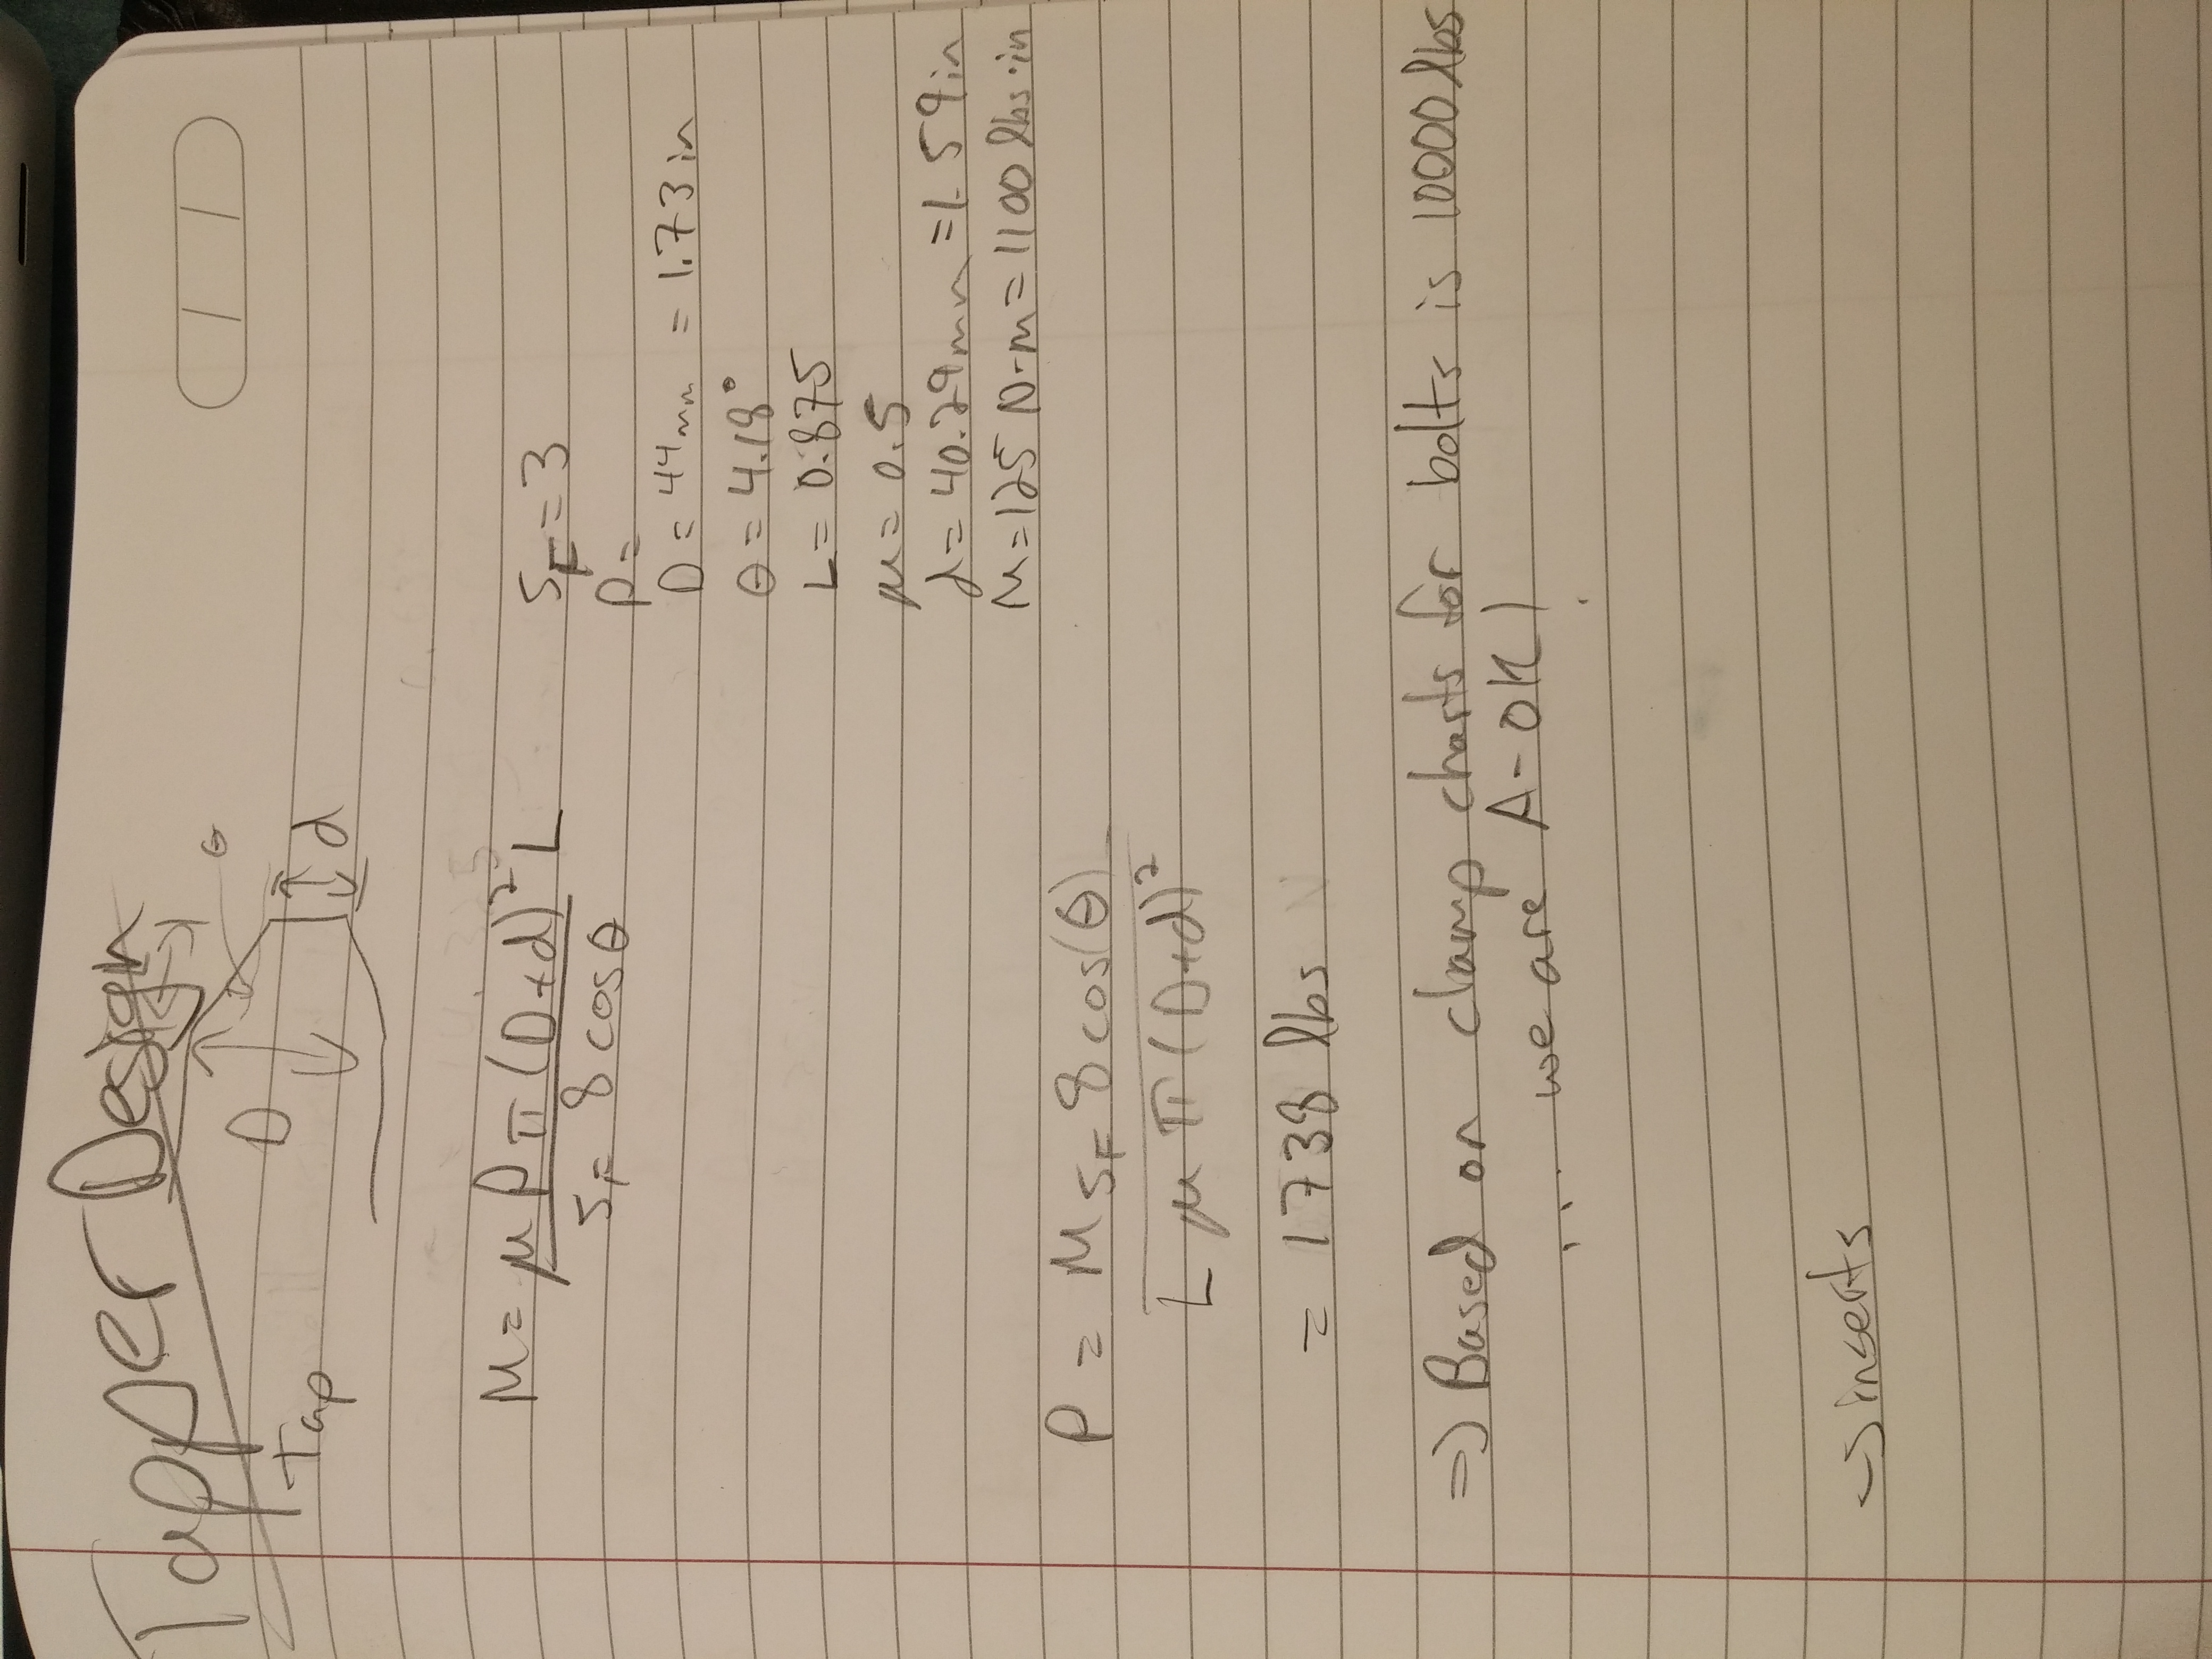
\includegraphics[width=\textwidth]{dom/taper_design_calc.jpg}
	\caption{Taper Mount Design Calculations}
	\label{fig:taper_calc}
\end{figure}

\begin{figure}[H]
\centering
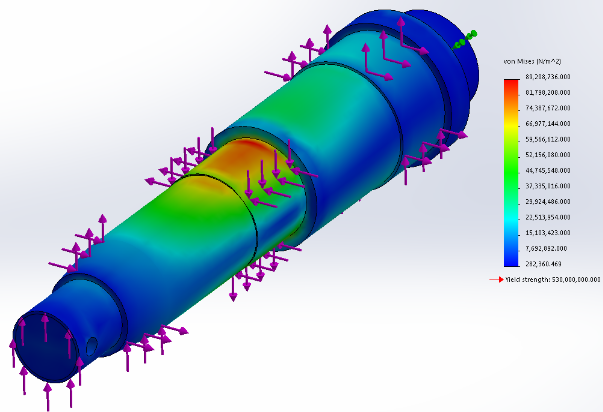
\includegraphics[width=\textwidth]{images/wheel_shaft_fea}
\caption[Wheel Shaft FEA Stress Results]{FEA stress results for wheel shaft. Maximum stress is 81 MPa}
\label{fig:wheel_shaft_stress_fea}
\end{figure}

\subsection{Wheel Bearings}\label{sec:ws_bearing}

\begin{figure}[H]
	\centering
	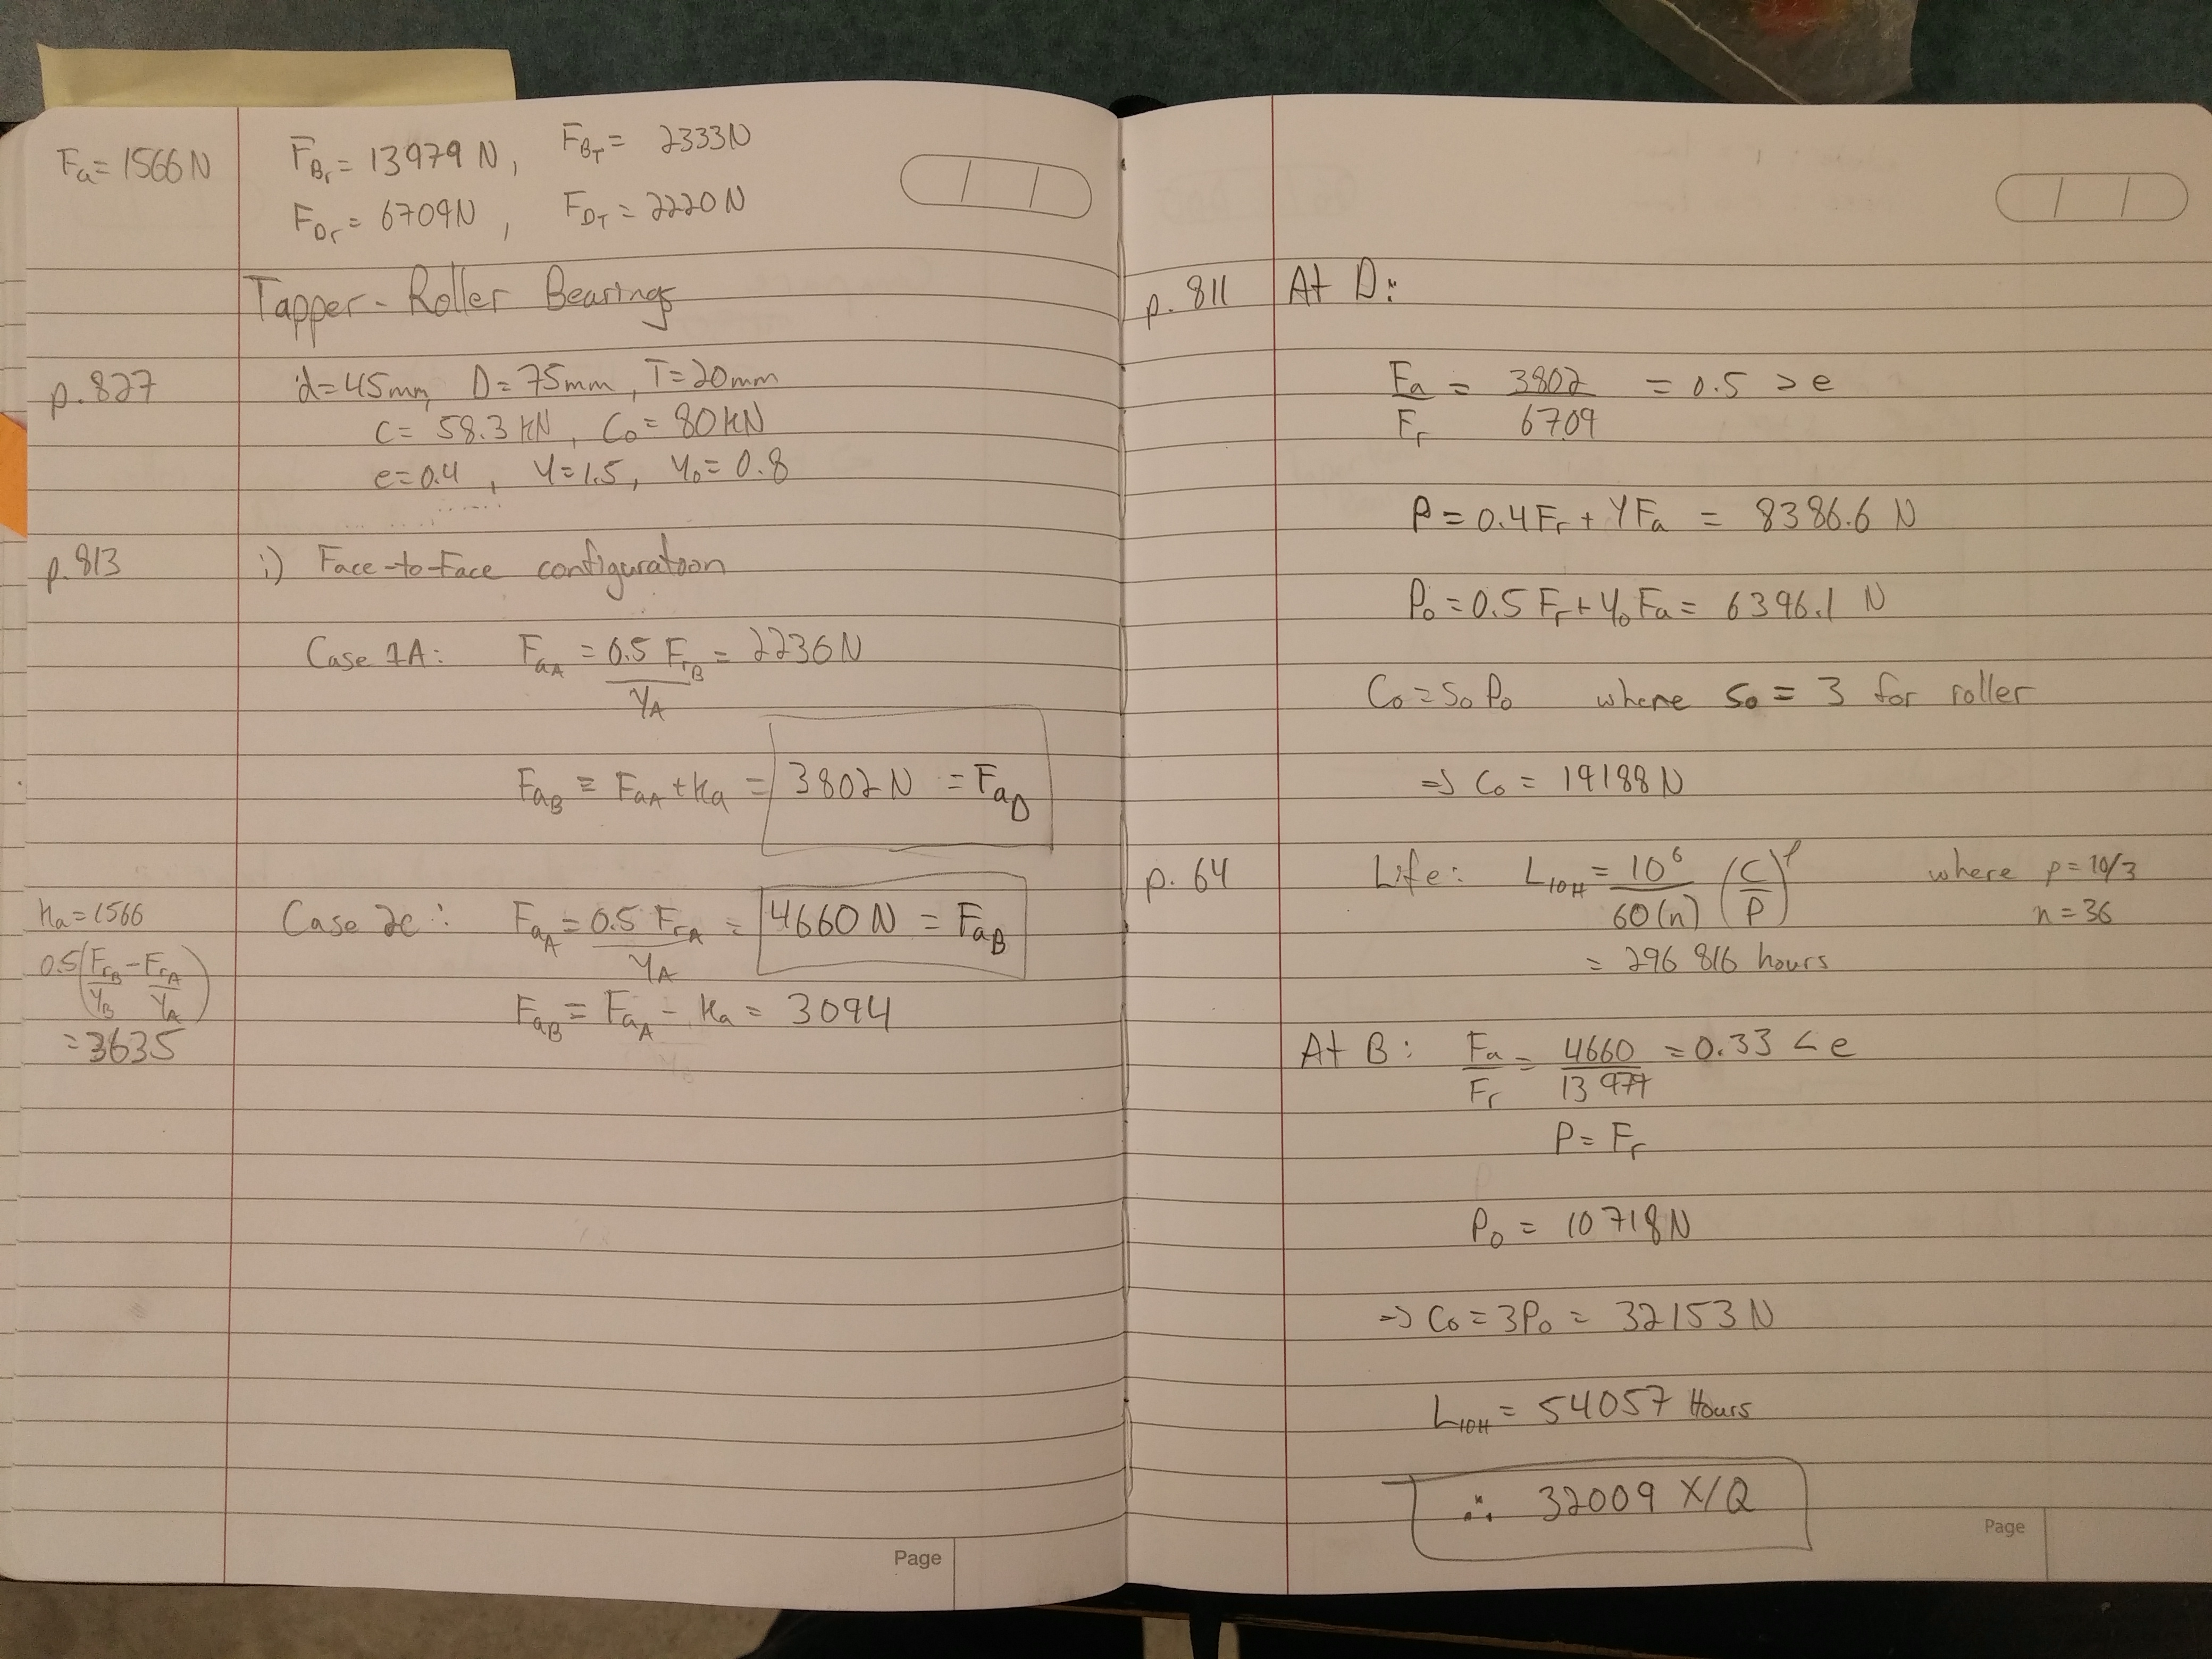
\includegraphics[width=\textwidth]{dom/bearing_selection_calc.jpg}
	\caption{Sample calculation for bearing selection process.}
	\label{fig:bearing_calc}
\end{figure}

\subsection{Bearing Housing}\label{sec:bh_fea}

\begin{figure}[H]
\centering
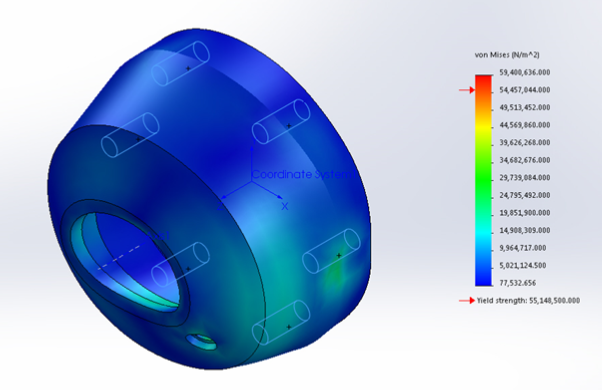
\includegraphics[width=\textwidth]{images/wheel_hub_fea}
\caption[Wheel Bearing Housing FEA Stress Results]{FEA stress results for wheel bearing housing. Maximum stress is 59 MPa}
\label{fig:wheel_hub_stress_fea}
\end{figure}


\subsection{Drive Shaft}\label{sec:drive_shaft_fea}

\begin{figure}[H]
\centering
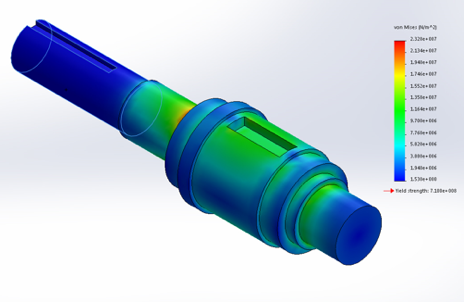
\includegraphics[width=\textwidth]{images/FEA_driveShaft}
\caption[Drive Shaft FEA Stress Results]{FEA stress results for drive shaft. Maximum stress is 23 MPa}
\label{fig:wheel_shaft_stress_fea}
\end{figure}

\subsection{Pivot}\label{sec:pivot_fea}

\begin{figure}[H]
\centering
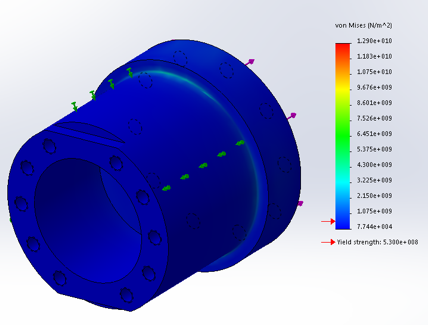
\includegraphics[width=0.9\textwidth]{images/FEA_pivotfinal}
\caption[Pivot FEA Stress Results]{FEA stress results for pivot analysis.}
\label{fig:pivot_stress_fea}
\end{figure}

\begin{figure}[H]
\centering
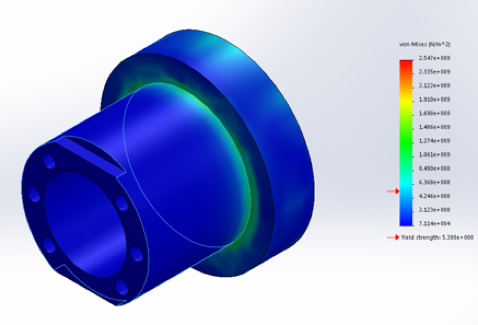
\includegraphics[width=0.9\textwidth]{images/FEA_pivotold}
\caption[Pivot FEA Stress Results]{FEA stress results for pivot analysis.}
\label{fig:old_pivot_stress_fea}
\end{figure}


\subsection{Drive Box}\label{sec:box_fea}

\begin{figure}[H]
\centering
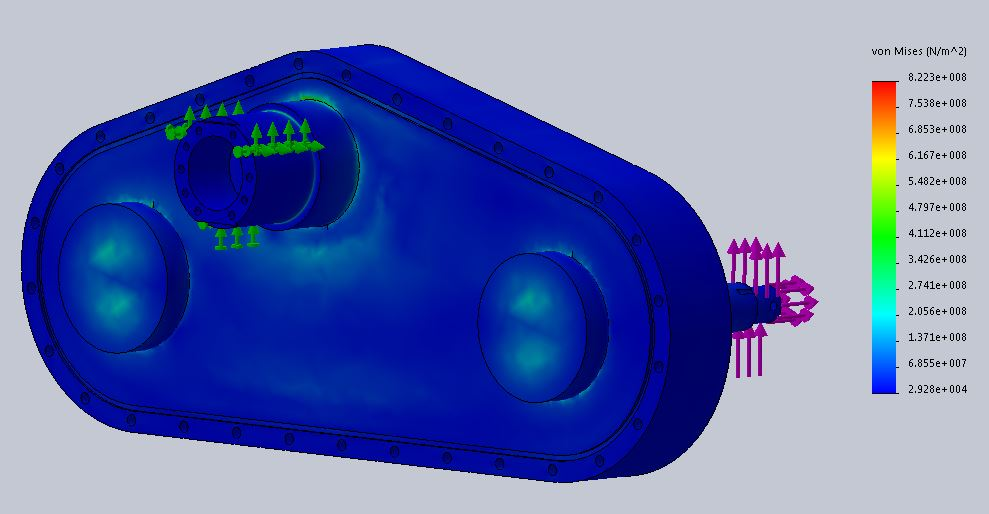
\includegraphics[width=\textwidth]{images/drive_box_stress_fea}
\caption[Drive Box FEA Stress Results]{FEA stress results for drive box analysis. Maximum stress is 82.23 MPa.}
\label{fig:box_fea1}
\end{figure}

\begin{figure}[H]
\centering
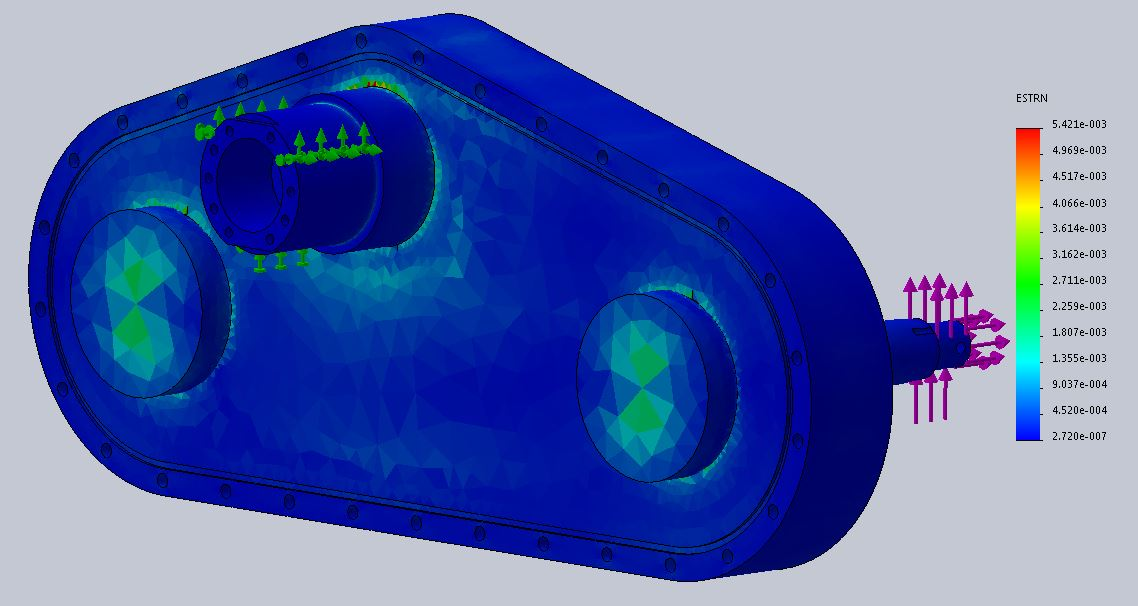
\includegraphics[width=\textwidth]{images/drive_box_strain_fea}
\caption[Drive Box FEA Strain Results]{FEA strain results for drive box analysis. Maximum strain is 5 mm.}
\label{fig:box_fea2}
\end{figure}

\subsection{Tensioner}\label{sec:idler_fea}

\begin{figure}[H]
\centering
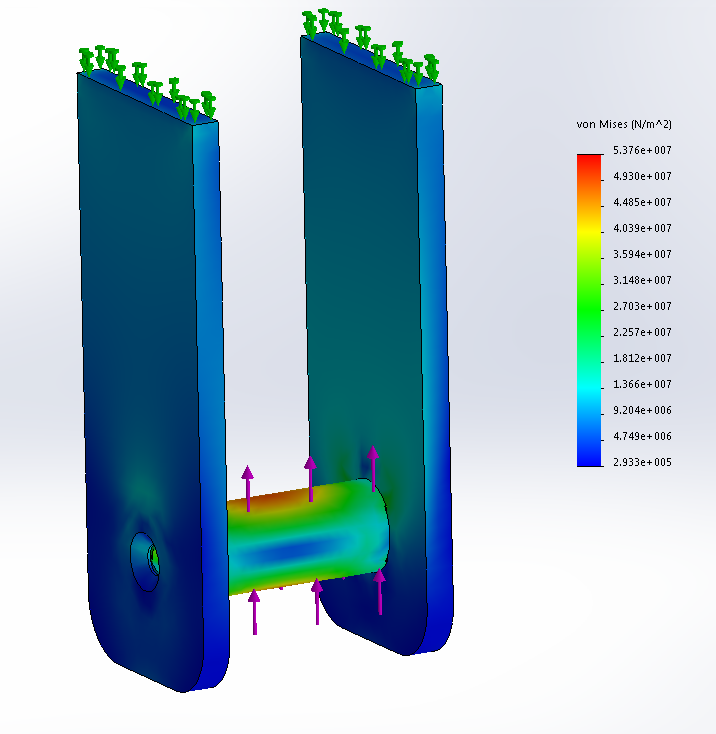
\includegraphics[width=\textwidth]{images/tensioner_vonmises_fea}
\caption[Tensioner FEA Stress Results]{FEA stress results for tensioner analysis. Maximum stress is 53.6 MPa.}
\label{fig:idler_fea1}
\end{figure}

\begin{figure}[H]
\centering
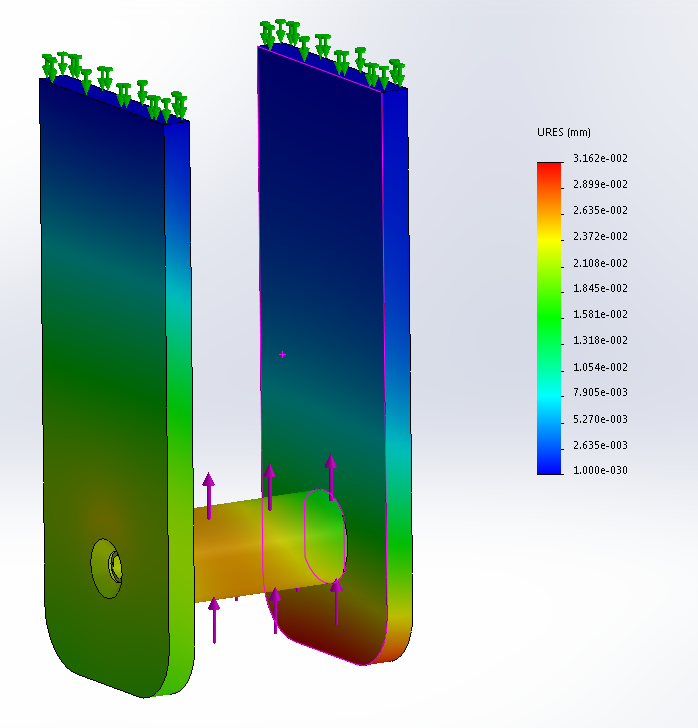
\includegraphics[width=\textwidth]{images/tensioner_displacement_fea}
\caption[Tensioner FEA Displacement Results]{FEA displacement results for tensioner analysis. Maximum displacement is 0.03 mm.}
\label{fig:idler_fea2}
\end{figure}

\subsection{Battery Rack}\label{sec:br_fea}

\begin{figure}[H]
\centering
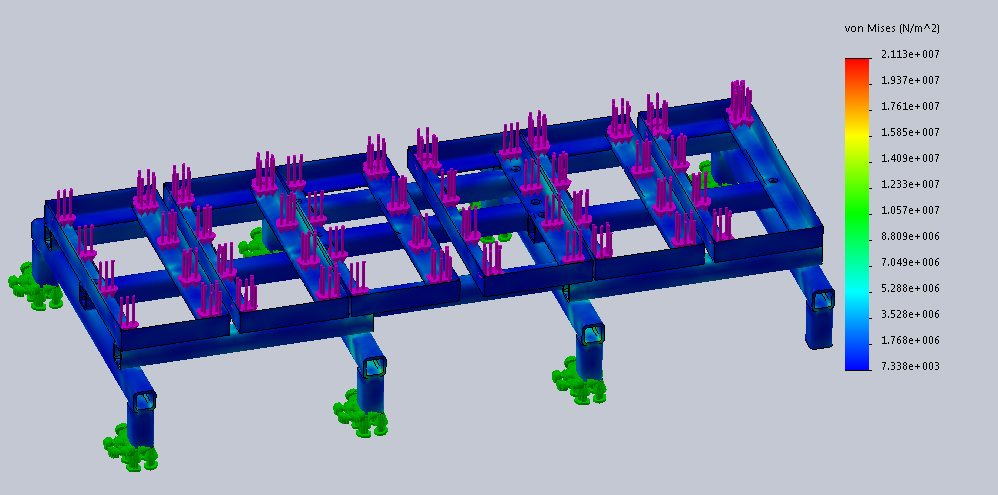
\includegraphics[width=\textwidth]{images/updated_battery_rack_VM}
\caption[Battery Rack FEA Stress Results]{FEA stress results for battery rack analysis. Maximum stress is 21.1 MPa.}
\label{fig:battery_rack_stress_fea}
\end{figure}

\begin{figure}[H]
\centering
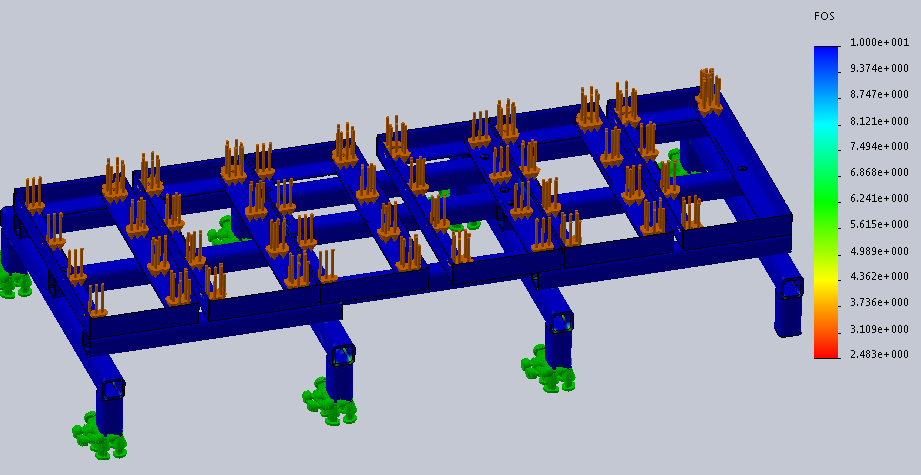
\includegraphics[width=\textwidth]{images/updated_battery_rack_FOS}
\caption[Battery Rack FEA factor of safety Results]{FEA factor of safety results for battery rack analysis. The smallest factor of safety is 2.5.}
\label{fig:battery_rack_disp_fea}
\end{figure}


